\documentclass[tikz,border=0pt]{standalone}
\usepackage{fontspec}
\hyphenpenalty=10000
\exhyphenpenalty=10000
\setmainfont[Path=../fonts/,BoldFont=Poppins-SemiBold.ttf,ItalicFont=Poppins-Italic.ttf]{Poppins-Regular.ttf}
\usepackage{pgfplots}
\pgfplotsset{compat=1.18}
\usetikzlibrary{calc,arrows.meta}
\definecolor{ink}{HTML}{161b22}
\definecolor{text}{HTML}{353535}
\definecolor{muted}{HTML}{646c74}
\definecolor{line}{HTML}{d7dadd}
\definecolor{wash}{HTML}{f6f6f6}
\definecolor{tint}{HTML}{e6ecef}
\definecolor{link}{HTML}{1d63b7}
\definecolor{local}{HTML}{376c97}
\definecolor{api}{HTML}{995d46}
\definecolor{cloud}{HTML}{7b649b}
\definecolor{match}{HTML}{7d9fc4}
\definecolor{miss}{HTML}{e0e3e5}
\begin{document}
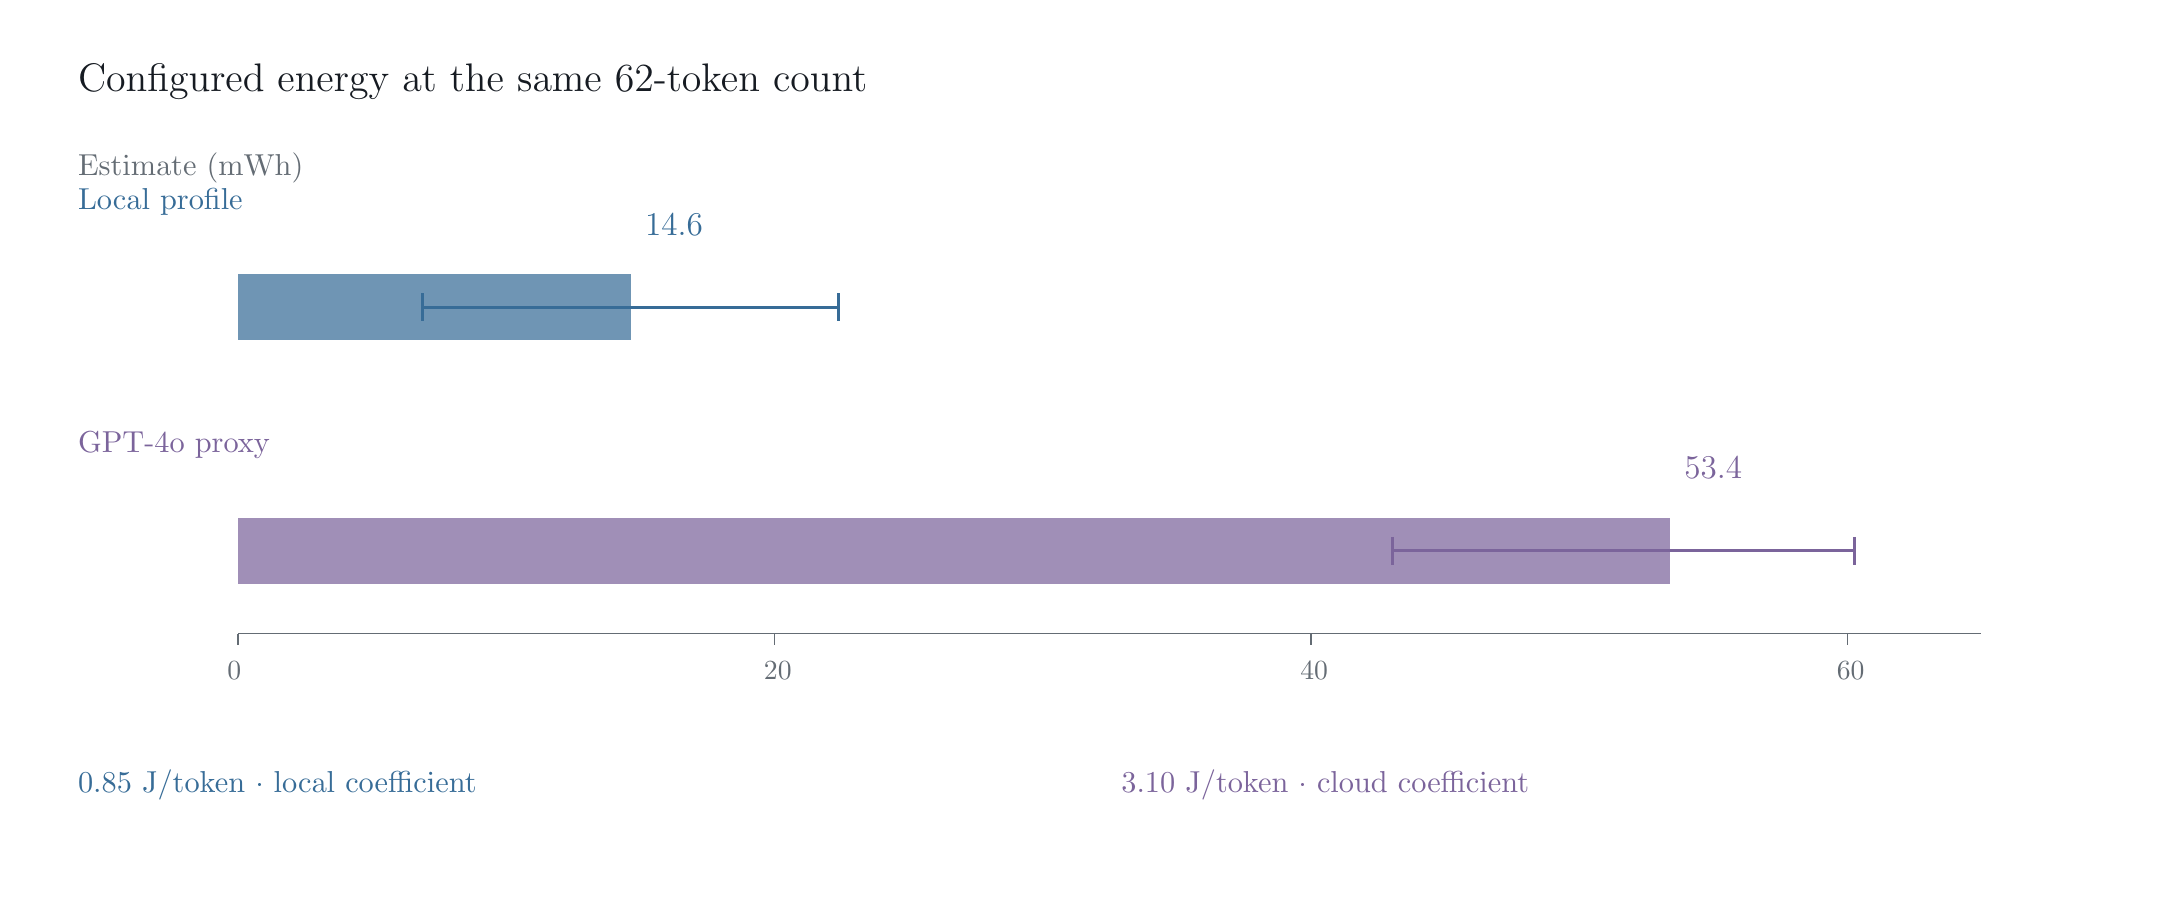
\begin{tikzpicture}[x=1pt,y=-1pt]
\path[use as bounding box] (0,0) rectangle (760,310);
\node[anchor=north west,inner sep=0pt,text=ink,align=left,font=\fontsize{14}{21.0}\selectfont,text width=724pt] at (18,13) {Configured energy at the same 62-token count};
\node[anchor=north west,inner sep=0pt,text=muted,align=left,font=\fontsize{10.5}{15.75}\selectfont] at (18,45) {Estimate (mWh)};
\node[anchor=north west,inner sep=0pt,text=local,align=left,font=\fontsize{11}{16.5}\selectfont] at (18,58) {Local profile};
\path[fill=local!72!white] (76,89) rectangle (217.885,113);
\draw[local,line width=1pt] (142.769,101) -- (293.000,101);
\draw[local,line width=1pt] (142.769,96) -- (142.769,106);
\draw[local,line width=1pt] (293.000,96) -- (293.000,106);
\node[anchor=north west,inner sep=0pt,text=local,align=left,font=\fontsize{12}{18.0}\selectfont] at (222.88461538461536,67) {14.6};
\node[anchor=north west,inner sep=0pt,text=cloud,align=left,font=\fontsize{11}{16.5}\selectfont] at (18,146) {GPT-4o proxy};
\path[fill=cloud!72!white] (76,177) rectangle (593.462,201);
\draw[cloud,line width=1pt] (493.308,189) -- (660.231,189);
\draw[cloud,line width=1pt] (493.308,184) -- (493.308,194);
\draw[cloud,line width=1pt] (660.231,184) -- (660.231,194);
\node[anchor=north west,inner sep=0pt,text=cloud,align=left,font=\fontsize{12}{18.0}\selectfont] at (598.4615384615385,155) {53.4};
\draw[muted,line width=.5pt] (76,219) -- (706,219);
\draw[muted,line width=.5pt] (76.0,219) -- (76.0,223);
\node[anchor=north west,inner sep=0pt,text=muted,align=left,font=\fontsize{10}{15.0}\selectfont] at (72.0,229) {0};
\draw[muted,line width=.5pt] (269.8461538461538,219) -- (269.8461538461538,223);
\node[anchor=north west,inner sep=0pt,text=muted,align=left,font=\fontsize{10}{15.0}\selectfont] at (265.8461538461538,229) {20};
\draw[muted,line width=.5pt] (463.6923076923077,219) -- (463.6923076923077,223);
\node[anchor=north west,inner sep=0pt,text=muted,align=left,font=\fontsize{10}{15.0}\selectfont] at (459.6923076923077,229) {40};
\draw[muted,line width=.5pt] (657.5384615384615,219) -- (657.5384615384615,223);
\node[anchor=north west,inner sep=0pt,text=muted,align=left,font=\fontsize{10}{15.0}\selectfont] at (653.5384615384615,229) {60};
\node[anchor=north west,inner sep=0pt,text=local,align=left,font=\fontsize{11}{16.5}\selectfont] at (18,268) {0.85 J/token · local coefficient};
\node[anchor=north west,inner sep=0pt,text=cloud,align=left,font=\fontsize{11}{16.5}\selectfont] at (395,268) {3.10 J/token · cloud coefficient};

\end{tikzpicture}
\end{document}
